\section{RP14 Unobtrusive JavaScript}
\label{sec:principle-rp14-unobtrusive-javascript}

Aktuelle Webapplikationen können grob in zwei Kategorien eingeteilt werden:

\begin{figure}[H]
	\begin{table}[H]
		\tablestyle
		\tablealtcolored
		\begin{tabularx}{\textwidth}{l l X}
			\tableheadcolor
				\tablehead Kategorie &
				\tablehead Beispiel &
				\tablehead Erläuterung
				\tabularnewline
			\tablebody
				Statisch &
				\emph{GitHub} \cite{GitHub} &
				User Interface wird auf dem Server gerendert, JavaScript bringt lediglich dynamisch geladene Inhalte, Effekte oder zusätzliche ``optionale'' Features.
				\tabularnewline

				JavaScript Client &
				\emph{Google Drive} \cite{GoogleDrive} &
				User Interface wird komplett im Browser mittels JavaScript aufgebaut. Ohne JavaScript keine Funktionalität oder schlechtere User Experience.
				\tabularnewline
			\tableend
		\end{tabularx}
	\end{table}
	\caption{Kategorisierung aktueller Webapplikationen}
	\label{tab:current-webapplication-categories}
\end{figure}

Die Kategorie \emph{Statisch} zeichnet sich durch eine hohe Kompatibilität mit allen möglichen Internetbrowsern aus. Durch die Generierung des HTML Markups losgelöst vom schlussendlichen Zielclient, liegt die ganze Verantwortung, vom beschaffen anzuzeigender Daten bis hin zum zusammenstellen des HTML \gls{DOM}'s komplett bei der Serverkomponente.

Zwar kommt auch bei diesem Typus oftmals JavaScript zur Anwendung, meist beschränkt sich dessen Anwendung aber auf die Ergänzung des bereits statisch geladenen Inhaltes. So lädt \emph{Mila} \cite{Mila} beim Seitenwechsel, sofern JavaScript aktiviert, neuen Inhalt über einen \gls{AJAX} Request. Nach Erhalt des vorgerenderten HTML Markups aus der Antwort ersetzt es entsprechende Inhalte im aktuell angezeigten HTML \gls{DOM} des Browsers.

Als Programmiersprache auf dem Applikationsserver kommt hier oft Java, Python, PHP, Ruby o.Ä. zum Einsatz.

Beim puren \emph{JavaScript Client} liegt der Programmcode für das Rendern des User Interfaces mit all seinen Inhalten als JavaScript Quelltext vor. Nach erfolgreicher Übertragung zum Internetbrowser initiiert dieser die Erstellung der Applikationsoberfläche im HTML \gls{DOM} des Clients.

Sollen dynamische Informationen angezeigt werden, müssen diese über eine Serviceschnittstelle beim entsprechenden Anbieter angefragt werden (siehe bspw. Abschnitt \ref{sec:principle-rp1-rest} ``\nameref{sec:principle-rp1-rest}'').

Die Verlagerung des User Interface Quelltexts direkt in den Browser hat den Vorteil, dass UI Element effizienter verändert und aktualisiert werden können. Möchten wir bspw. Informationen aus einem Webservice in einer Tabelle anzeigen lassen, können wir diese einmalig laden. Zur effektiven Anzeige muss keine weitere Anfrage an die Backendkomponente getätigt werden, um die bezogenen Informationen in HTML Markup umwandeln zu lassen. Der bereits im Browser verfügbare JavaScript Code übernimmt diese Aufgabe.

Durch diese Vereinfachung entfallen unnötige Wartezeiten zwischen Benutzereingabe und Systemreaktion. Dies resultiert wiederum in einer verbesserten User Experience.

Es ist bereits zu erahnen, dass diese Art von Webapplikation ohne JavaScript-Unterstützung im Browser des Endbenutzers nicht ausgeführt werden kann. Ein Beispiel hierfür liefert der \emph{Google Drive} \cite{GoogleDrive} Webclient. Wie in Abbildung \ref{fig:googleDriveNoJs} ersichtlich verweigert dieser ohne aktiviertes JavaScript die Funktion und zeigt ein leeres Standardlayout mit einer entsprechenden Meldung an.

\begin{figure}[H]
	\centering
	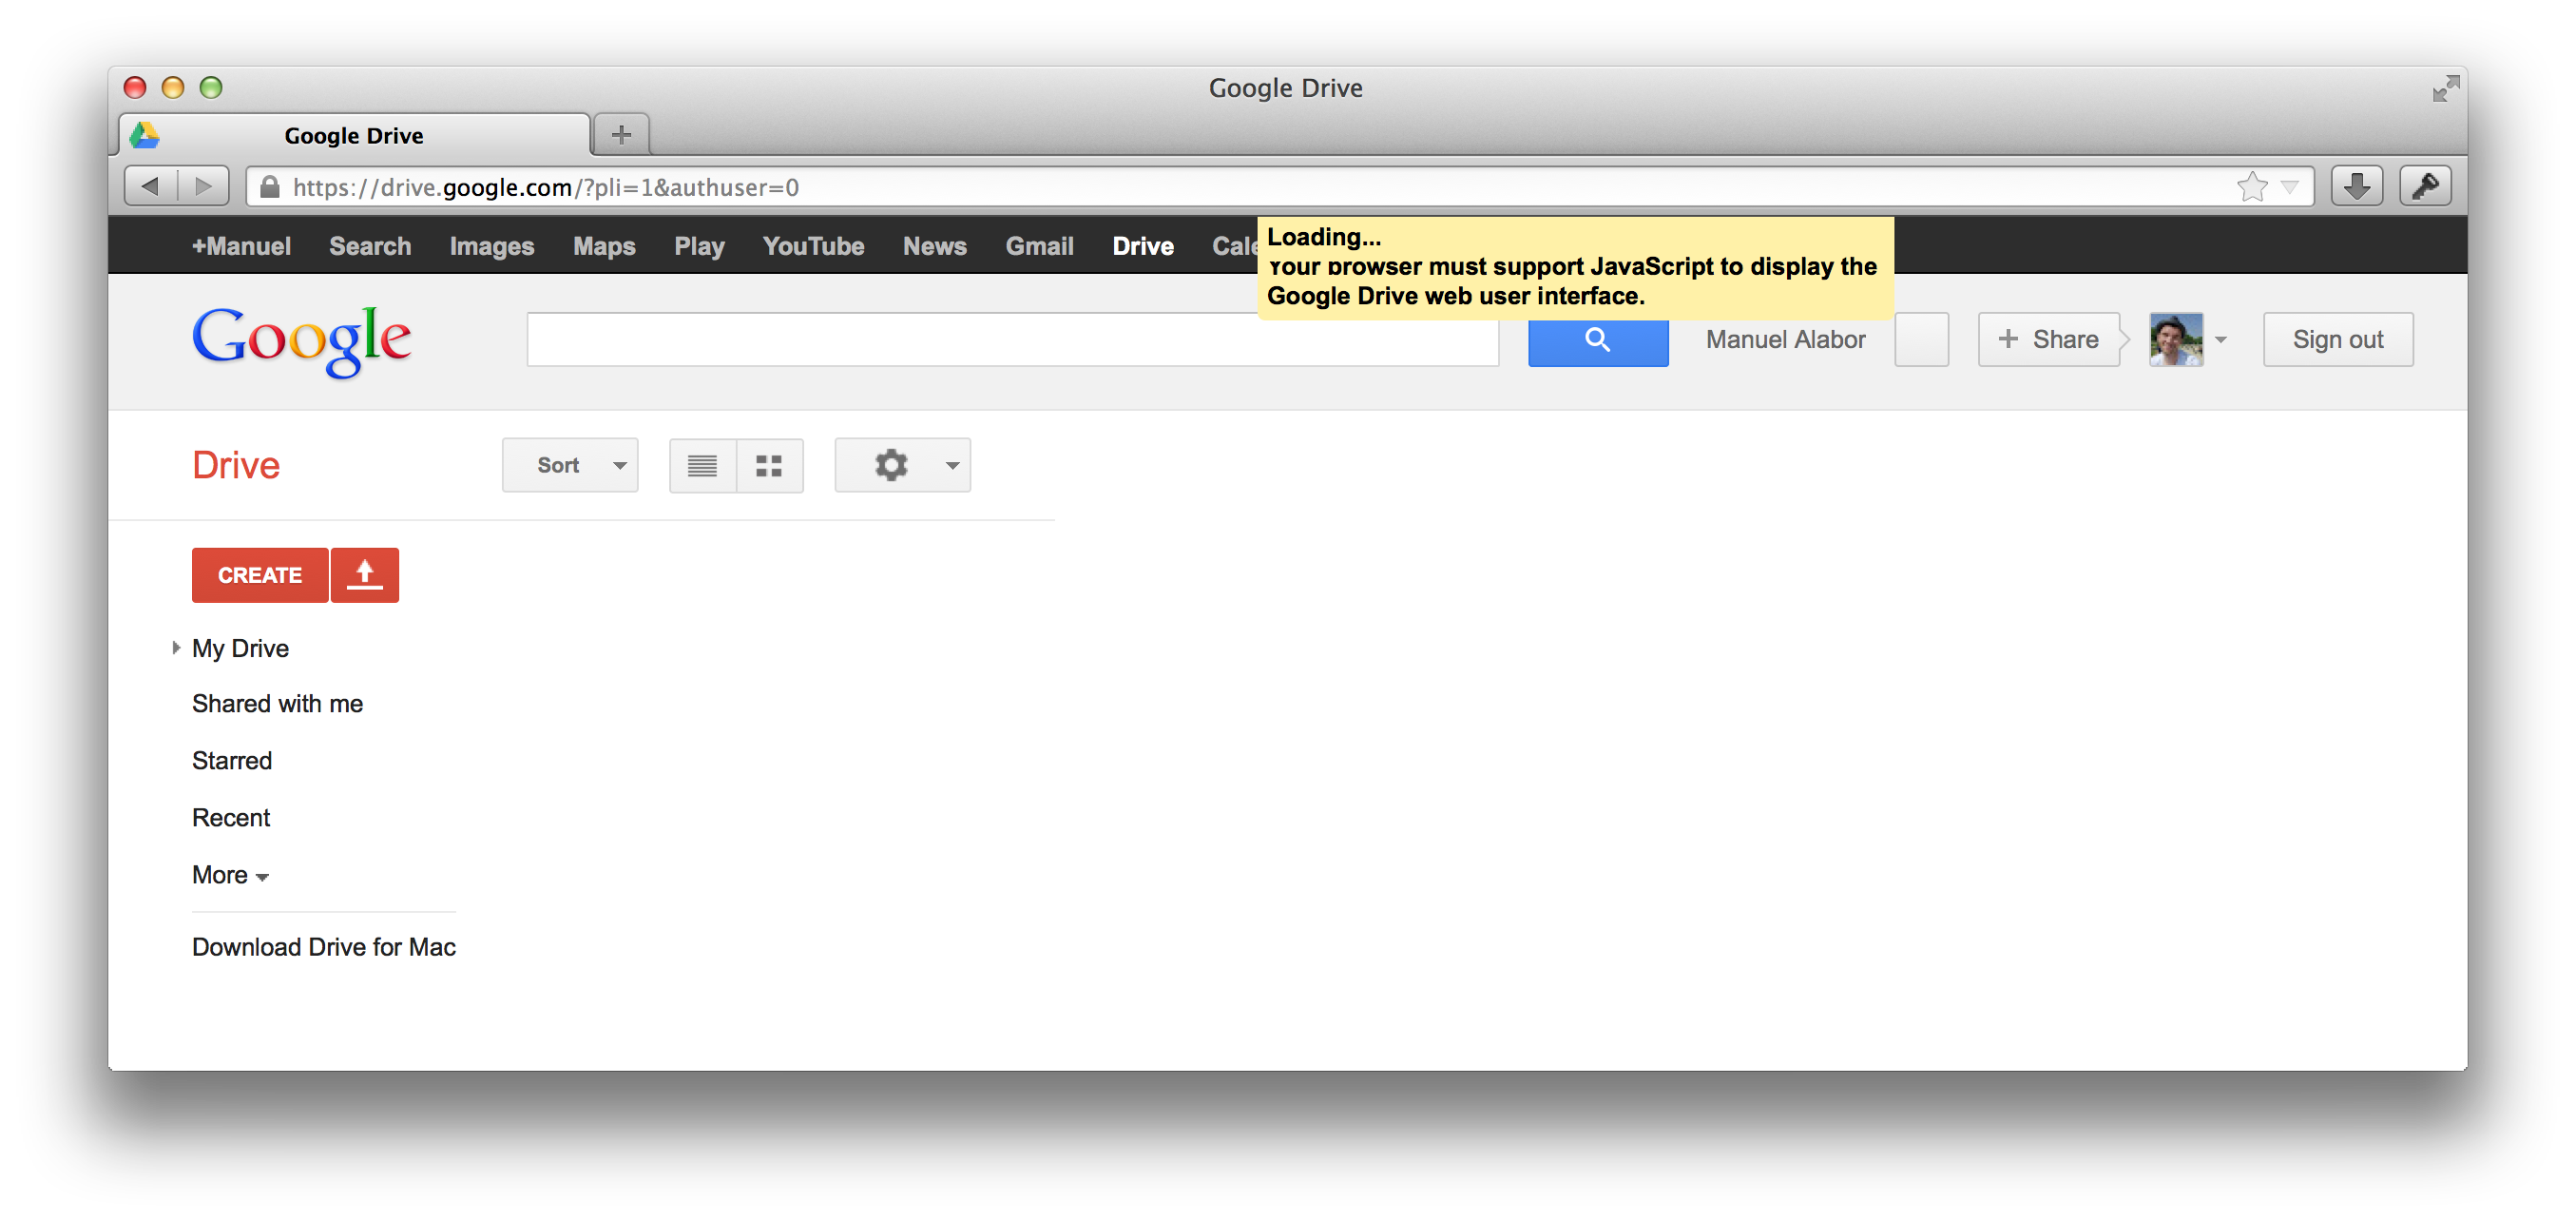
\includegraphics[width=12cm]{content/principle-demonstration/images/googledrive-nojs.png}
	\caption{\emph{Google Drive} in Firefox 21.0 mit deaktiviertem JavaScript}
	\label{fig:googleDriveNoJs}
\end{figure}

Die Richtlinie \emph{RP14 Unobtrusive JavaScript} aus dem ROCA Manifest verlangt, dass eine Webapplikation auch bei deaktiviertem JavaScript weiter funktionstüchtig bleibt. Konkret wünscht \emph{RP14} also eine Mischform aus den vorgestellten Applikationstypen.


\subsection*{Geplante Umsetzung}

Als Herausforderung hat das Projektteam geplant, die Beispielapplikation \emph{Roomies} als Mischform der im einleitenden Abschnitt vorgestellten Applikationstypen umzusetzen.

Grundsätzlich sollen Inhalte statisch auf der Backendkomponente gerendert werden. Hat der Benutzer in seinem Browser JavaScript aktiviert, ermöglicht entsprechender Programmcode die Umsetzung der im einleitenden Abschnitt vorgestellten Funktionalitäten eines vollwertigen \emph{JavaScript Clients}.

Zugriffe auf persistente Applikationsdaten sollen wie in \ref{sec:principle-rp1-rest} ``\nameref{sec:principle-rp1-rest}'' vorgeschlagen in ein entkoppeltes Serviceinterface gekapselt werden.


\subsection*{Konkrete Umsetzung}

Während der Implementation der geplanten Lösung wurde sehr schnell klar, das die entstehende Applikation zwar wie erwartet die gewünschte hybride Form aufweisen wird, aber keinesfalls mit der ROCA Richtlinie \emph{\nameref{sec:principle-rp15-no-duplication}} vereinbar sein wird.

Zwar hätten viele Codefragmente wie die View-Templates (Beispiel siehe Quelltext \ref{lst:reusableHandlebarsViewTemplate}) dank der durchgängigen Verwendung von JavaScript auch im Frontend wiederverwendet werden können. Andere, logikintensivere Komponenten wie die Controller zur Steuerung der eigentlichen User Interface Funktionalitäten (Event-Handling, Datenzugriffe etc.) hätten doppelt implementiert werden müssen.

\begin{lstlisting}[language=JavaScript, firstnumber=31, caption={Ausschnitt aus dem \emph{Handlebars} \cite{Handlebars} Template zur Darstellung von Benutzerinformation in der Menüleiste von \emph{Roomies} \cite{roomiesMenuTemplate}}, label={lst:reusableHandlebarsViewTemplate}]
{{#if user}}
<ul class="right">
	<li class="account">
		<a href="/resident/{{user.facebookId}}/profile">
			<span class="item-label">{{user.name}}</span>
			<img class="avatar small" src="//graph.facebook.com/{{user.facebookId}}/picture" />
		</a>
	</li>
</ul>
{{/if}}
\end{lstlisting}

Um diesem Umstand gegensteuern zu können teilte sich das Projektteam nach der ersten Entwicklungsiteration in zwei Gruppen:

\begin{itemize}
	\item Zwei Mitglieder arbeiteten weiter an der Umsetzung der geplanten Use Cases
	\item Ein Mitglied fokussierte sich auf die Entwicklung einer Möglichkeit, identischen Applikationscode sowohl in der Backend-Komponente für statisches Rendering als auch direkt im Browser als JavaScript Client verwenden zu können.
\end{itemize}

Aus diesem Prozess entstand das eigenständige Framework \emph{barefoot} \cite{Barefoot}. Es setzt auf der verbreiteten Bibliothek \emph{Backbone.js} \cite{Backbonejs} auf und ermöglicht die Verwendung einer einzigen, einheitlichen Codebasis für JavaScript-basierte Webapplikationen.

Mit der Integration des neuartigen Frameworks kann erstmals komplett auf doppelte Codefragmente verzichtet werden. Gleichzeitig profitiert der Endbenutzer von kurzen Lade- und Reaktionszeiten im User Interface. Sollte auf einem Client kein JavaScript verfügbar sein, greift automatisch das klassische servergestützte Rendering und alle Funktionalitäten bleiben zugänglich.


\subsection*{Diskussion}


